%%%%%%%%%%%%%%%%%%%%%%%%%%%%%%%%%%%%%%%%%
% kaobook
% LaTeX Template
% Version 1.2 (4/1/2020)
%
% This template originates from:
% https://www.LaTeXTemplates.com
%
% For the latest template development version and to make contributions:
% https://github.com/fmarotta/kaobook
%
% Authors:
% Federico Marotta (federicomarotta@mail.com)
% Based on the doctoral thesis of Ken Arroyo Ohori (https://3d.bk.tudelft.nl/ken/en)
% and on the Tufte-LaTeX class.
% Modified for LaTeX Templates by Vel (vel@latextemplates.com)
%
% License:
% CC0 1.0 Universal (see included MANIFEST.md file)
%
%%%%%%%%%%%%%%%%%%%%%%%%%%%%%%%%%%%%%%%%%

%----------------------------------------------------------------------------------------
%	PACKAGES AND OTHER DOCUMENT CONFIGURATIONS
%----------------------------------------------------------------------------------------

\documentclass[
	fontsize=11pt, % Base font size
	twoside=true, % Use different layouts for even and odd pages (in particular, if twoside=true, the margin column will be always on the outside)
	%open=any, % If twoside=true, uncomment this to force new chapters to start on any page, not only on right (odd) pages
	%chapterprefix=true, % Uncomment to use the word "Chapter" before chapter numbers everywhere they appear
	%chapterentrydots=true, % Uncomment to output dots from the chapter name to the page number in the table of contents
	numbers=noenddot, % Comment to output dots after chapter numbers; the most common values for this option are: enddot, noenddot and auto (see the KOMAScript documentation for an in-depth explanation)
	%draft=true, % If uncommented, rulers will be added in the header and footer
	%overfullrule=true, % If uncommented, overly long lines will be marked by a black box; useful for correcting spacing problems
]{kaobook}

% Set the language
\usepackage[english]{babel} % Load characters and hyphenation
\usepackage[english=british]{csquotes} % English quotes

% Load packages for testing
\usepackage{blindtext}
%\usepackage{showframe} % Uncomment to show boxes around the text area, margin, header and footer
%\usepackage{showlabels} % Uncomment to output the content of \label commands to the document where they are used

% Load the bibliography package
\usepackage{styles/kaobiblio}
\addbibresource{main.bib} % Bibliography file

% Load mathematical packages for theorems and related environments. NOTE: choose only one between 'mdftheorems' and 'plaintheorems'.
\usepackage{styles/mdftheorems}
%\usepackage{styles/plaintheorems}

\graphicspath{{examples/documentation/images/}{images/}} % Paths in which to look for images

\makeindex[columns=2, title=Alphabetical Index, intoc] % Make LaTeX produce the files required to compile the index

\makeglossaries % Make LaTeX produce the files required to compile the glossary

\makenomenclature % Make LaTeX produce the files required to compile the nomenclature

% Reset sidenote counter at chapters
%\counterwithin*{sidenote}{chapter}

%----------------------------------------------------------------------------------------

\begin{document}

%----------------------------------------------------------------------------------------
%	BOOK INFORMATION
%----------------------------------------------------------------------------------------

\titlehead{ShEx-Lite}
\subject{Final Degree Project}

\title[ShEx-Lite]{ShEx-Lite}
\subtitle{Automatic generation of domain object models through a subset of a shape expressions language.}

\author[Guillermo Facundo Colunga]{Guillermo Facundo Colunga}

\date{\today}

\publishers{University of Oviedo}

%----------------------------------------------------------------------------------------

\frontmatter % Denotes the start of the pre-document content, uses roman numerals

%----------------------------------------------------------------------------------------
%	OPENING PAGE
%----------------------------------------------------------------------------------------

%\makeatletter
%\extratitle{
%	% In the title page, the title is vspaced by 9.5\baselineskip
%	\vspace*{9\baselineskip}
%	\vspace*{\parskip}
%	\begin{center}
%		% In the title page, \huge is set after the komafont for title
%		\usekomafont{title}\huge\@title
%	\end{center}
%}
%\makeatother

%----------------------------------------------------------------------------------------
%	COPYRIGHT PAGE
%----------------------------------------------------------------------------------------

\makeatletter
\uppertitleback{\@titlehead} % Header

\lowertitleback{
	Final Degree Project presented on July 2020 at the School of Software Engineering, Oviedo University. All the source code related to the implementation explored during this book is available at \url{github.com/weso/shex-lite}.
	
	\medskip
	
	\textbf{Copyright}\\
	All rights reserved. This project or any portion may not be reproduced or used in any manner without the express quotation to the original author.
	
	\medskip
	
	\textbf{Directors} \\
	Dr. Jose Emilio Labra Gayo\\Daniel Fernández Álvarez
}
\makeatother

%----------------------------------------------------------------------------------------
%	DEDICATION
%----------------------------------------------------------------------------------------

\dedication{
	The harmony of the world is made manifest in Form and Number, and the heart and soul and all the poetry of Natural Philosophy are embodied in the concept of mathematical beauty.\\
	\flushright -- D'Arcy Wentworth Thompson
}

%----------------------------------------------------------------------------------------
%	OUTPUT TITLE PAGE AND PREVIOUS
%----------------------------------------------------------------------------------------

% Note that \maketitle outputs the pages before here

% If twoside=false, \uppertitleback and \lowertitleback are not printed
% To overcome this issue, we set twoside=semi just before printing the title pages, and set it back to false just after the title pages
\KOMAoptions{twoside=semi}
\maketitle
\KOMAoptions{twoside=false}

%----------------------------------------------------------------------------------------
%	AKNOWLEDGEMENTS
%----------------------------------------------------------------------------------------

\chapter*{Aknowledgments}
\addcontentsline{toc}{chapter}{Aknowledgments} % Add the preface to the table of contents as a chapter

There are many people thanks to whom I write this work today. First of all I would like to thank my teachers Dr. Jose Emilio Labra Gayo and Daniel Fernández Álvarez, as well as the semantic web research group of the University of Oviedo for the trust placed in me to carry out this project.
However, this project is done as a summary of what has been my time at the university and a personal stage. That is why I would like to make a small dedication to those people who in one way or another have helped me to write this project today.
To my mother, Esther, for waiting until I was ready to leave us. To my uncle Andrés for being my guardian angel. To my grandparents, for giving me everything they had. To my coach Vic, who unwittingly has become a father to me. To Laura, the impossible girl. Ricardo, although I have never counted on you, you have always been. To Monica, for being you. To Pablo, without you I would not be who I am and I would never have finished this degree. To Álvaro, for letting me be your “manín". To Sari, for laughing at me when I needed it. To Cotito, for teaching me to accept myself. To Alejandro, for getting me out of my comfort zone. To Pablín, for being my prettiest doctor. To all my friends and family, those who I did not mention and those that I left along the way I dedicate this work to you for the moments you give me. And finally to my CAU family, thank you, really.
I hope that this work and I will not be a disappointment to any of you, really, each and every one of you are exceptional.

\begin{kaobox}[frametitle=Spanish]
	Son muchas las personas gracias a las que hoy escribo este trabajo. En primer lugar me gustaría agradecer a mis tutores Aquilino Juan Fuerte y Jose Emilio Labra Gayo, así como al grupo de investigación de web semántica de la Universidad de Oviedo y a Izertis S.A. la confianza depositada en mi para la realización de este proyecto.
	Sin embargo este proyecto se realiza como resumen de lo que ha sido mi paso por la universidad y por una etapa personal. Es por eso que me gustaría realizar una pequeña dedicatoria a aquellas personas que de una forma u otra han ayudado a que este escribiendo este proyecto hoy. A mi madre, Esther, por esperar a que estuviera preparado para marcharse. A mi tío Andrés por haber sido mi angel de la guarda. A mis abuelos, por dejarse la vida en mí. A mi entrenador Vic, quien sin quererlo se ha convertido en un padre. A Laura, la chica imposible. A Ricardo, aunque jamás he contado contigo siempre has estado. A Mónica, por ser tú. A Pablo, sin ti no sería quién soy y jamás habría terminado la carrera. A Álvaro, por dejarme ser tu manín. A Sari, por reñirme cuando lo necesitaba. A Cotito, por ser enseñarme a aceptarme. A Alejandro, por sacarme de mi zona de confort. A Pablín, por ser mi médico más cuqui. A todos mis amigos y amigas que dejé por el camino os dedico este trabajo por los momentos que me distéis. Y finalmente a mi familia del CAU, gracias, de verdad.
	Espero que este trabajo y yo no seamos una decepción para ninguno de vosotros, de verdad, todos y cada uno sois excepcionales.
\end{kaobox}

%----------------------------------------------------------------------------------------
%	ABSTRACT
%----------------------------------------------------------------------------------------

\chapter*{Abstract}
\addcontentsline{toc}{chapter}{Abstract} % Add the preface to the table of contents as a chapter

This end of degree project is about creating a compiler for a subset of the Shape Expressions Compact Syntax, focused on syntactic and semantic validation and the generation of domain models in object oriented languages. \todo{Completar...}


%----------------------------------------------------------------------------------------
%	TABLE OF CONTENTS & LIST OF FIGURES/TABLES
%----------------------------------------------------------------------------------------

\begingroup % Local scope for the following commands

% Define the style for the TOC, LOF, and LOT
%\setstretch{1} % Uncomment to modify line spacing in the ToC
%\hypersetup{linkcolor=blue} % Uncomment to set the colour of links in the ToC
\setlength{\textheight}{23cm} % Manually adjust the height of the ToC pages

% Turn on compatibility mode for the etoc package
\etocstandarddisplaystyle % "toc display" as if etoc was not loaded
\etocstandardlines % toc lines as if etoc was not loaded

\tableofcontents % Output the table of contents

\listoffigures % Output the list of figures

% Comment both of the following lines to have the LOF and the LOT on different pages
\let\cleardoublepage\bigskip
\let\clearpage\bigskip

\listoftables % Output the list of tables

\endgroup

%----------------------------------------------------------------------------------------
%	MAIN BODY
%----------------------------------------------------------------------------------------

\mainmatter % Denotes the start of the main document content, resets page numbering and uses arabic numbers
\setchapterstyle{kao} % Choose the default chapter heading style

\chapter{Introduction}
\label{ch:intro}

This chapter covers the motivation, contributions and structure of the document.
The main objective of this chapter, therefore, is that after reading it, the reader
builds an idea about the motivations that have promoted this project, what is
being worked on and the contributions emanating from it.

% S E C T I O N   M O T I V A T I O N

\section{Motivation}
\label{sec:intro-motiv}

Each day, more and more devices generate data both automatically and manually, and also each day the development of
applications in different domains that are backed by databases and expose these data to the web becomes easier. The
amount and diversity of data produced clearly exceeds our capacity to consume it.

To describe the data that is so large and complex that traditional data processing applications can’t handle the
term Big Data \cite{big-data,sagiroglu2013big} has emerged. Big Data has been described by at least three words starting
by V: volume, velocity, variety. Although volume and velocity are the most visible features, variety is a key concept
which prevents data integration and generates lots of interoperability problems.

RDF \textit{(Resource Description Framework)} was proposed as a graph-based data model
\cite{graph-data-model} which became part of the Semantic Web \cite{semantic-web} vision.
Its reliance on the global nature of URIs\footnote{A Uniform Resource Identifier (URI) is a string of
characters that unambiguously identifies a particular resource. To guarantee uniformity, all URIs follow a predefined
set of syntax rules, but also maintain extensibility through a separately defined hierarchical naming scheme.
Ref.\url{https://en.wikipedia.org/wiki/Uniform_Resource_Identifier}} offered a solution to the data integration
problem as RDF datasets produced by different means can seamlessly be integrated with other data.

Related to this, is the concept of Linked Data \cite{linked-data} that was proposed as a set of best
practices to publish data on the Web. It was introduced by Tim Berners-Lee and was based on four main principles,
as mentioned in \cite{linked-data}:

\begin{itemize}
  \item Use URIs as names for things.
  \item Use HTTP URIs so that people can look up those names.
  \item When someone looks up a URI, provide useful information, using the standards (RDF, SPARQL).
  \item Include links to other URIs. so that they can discover more things.
\end{itemize}

\begin{figure}
    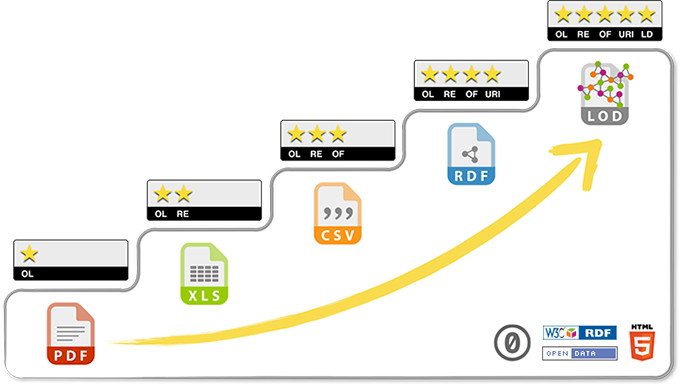
\includegraphics[scale=0.5]{images/5-star-steps.png}
    \centering
	\caption[The 5 star steps of Linked Data]{The 5 star steps of Linked Data.}
	\label{fig:margin-5-star-steps}
\end{figure}

Similar to this four principles is the 5 stars Linked Open Data Model, illustrated in \cref{fig:margin-5-star-steps}.
RDF is mentioned in the third principle as one of the standards that provides useful information. The goal of this
principles is that data is not only ready for humans to navigate through but also for other agents, like computers,
that may automatically process that data.

All the above motivations helped to make RDF the language for the Web of Data, as described in \cite{labra-validating-rdf}.
And the main features that it presents are: \textit{Disambiguation}, \textit{Integration}, \textit{Extensibility}, \textit{Flexibility} and \textit{Open by Default}.
With the features also some drawbacks are associated, the most important one and the one we will focus is the RDF
\textbf{production/consumption dilemma}.

RDF production/consumption dilemma states that it is necessary to find ways that data producers can generate their data so
it can be handled by potential consumers. For example, they may want to declare that some nodes have some properties with
some specific values. Data consumers need to know that structure to develop applications to consume the data.

Although RDF is a very flexible schema-less language, enterprise and industrial applications may require an extra level of
validation before processing for several reasons like security, performance, etc.

To solve that dilemma and as an alternative to expecting the data to have some structure without validation, Shape Expressions Language
\textit{(ShEx)} was proposed as a human-readable and high-level open source language for RDF validation. Initially, ShEx was proposed
as a human-readable syntax for OSLC Resource Shapes \cite{oslc-resource-shape} but ShEx grew very fast to embrace more
complex user requirements coming from clinical and library use cases.

Another technology, SPARQL Inferencing Notation (SPIN) \cite{knublauch2011spin}, was used for RDF validation, principally in TopQuadrant’s TopBraid Composer. This technology, influenced
from OSLC Resource Shapes as well, evolved into both a private implementation and open source definition of the SHACL
\textit{(Shapes Constraint Language)}, which was adopted by the W3C Data Shapes Working Group.

From a user point of view the possibilities of ShEx are very large, from the smallest case to just validate a node with one property
to a scientific domain case where we need to validate the human genome\footnote{\url{https://github.com/geneontology/go-shapes}}. A language with such a number
of possibilities requires from a strong syntactic and semantic validation and that leads us to our first goal.

\begin{researchquestion}
  Determine how much the existing syntactic and semantic validation systems for shape expressions can be enhanced. And
  if existing systems can be enhanced propose a prototype that implement those enhancements.
\end{researchquestion}

Secondly and very related to programming languages, if we take the PopularitY of Programming Language \textit{(PYPL)} Index\footnote{\url{http://pypl.github.io/PYPL.html}}
from June 2020 we can see that more than half of the share is occupied by languages that support the object oriented paradigm. And therefore this paradigm
becomes the most used one. The aim of this paradigm is to model real world domains, according to \cite{wegner1990concepts}. That, in fact, is the same goal
that ShEx has, it allows to model real world domains with schemas, and validate existing data with them. Therefore our second goal relies on this and tries
to automatically transform shape expressions into object domain models coded in any language that supports the object oriented paradigm:

\begin{researchquestion}
  Determine till which point can we automatically translate existing shape expressions to object domain models. And
  propose a prototype capable of translating Shape Expressions to object domain models.
\end{researchquestion}

If this were possible it would not only imply that you could automate the creation of application domain models but that you could link the domain model that an
application uses with a domain model defined through Shape Expressions that describes the schema of a RDF data set.

\bigskip

To give answers to the questions posed in this section, we will limit our scope to the micro grammar of Shape Expressions, defined in
\footnote{\url{https://dcmi.github.io/dcap/shex_lite/micro-spec.html}}. This version is a strict subset of the complete ShEx grammar
and therefore any derived method or technology we can draw from it can automatically be applied to the full grammar.

% S E C T I O N   C O N T R I B U T I O N S

\section{Contributions}
\label{sec:intro-contri}
These are the major contributions of this dissertation:

\begin{enumerate}
  \item A parser for the ShEx micro Compact Syntax. There are already existing parsers for ShEx and they work for ShEx micro Compact Syntax
  as it is a subset of ShEx, but they accept more structures than the ones defined by ShEx micro Compact Syntax. We propose a parser that
  is only focused on ShEx micro Compact Syntax and therefore error and warning messages can be enhanced.
  
  \item Error and warning analyser for schemas. Existing approaches do not semantically validate the schemas, they
  only perform error detection by means of complex grammars and parsers. Our proposed system does semantically validate the schemas by means
  of a custom analyser that performs both syntactic and semantic analysis so it produces human-friendly errors and warnings that users can
  use to fix their schemas.

  \item Automatic translation of schemas into object domain models in \texttt{Java} and \texttt{Python}. The proposed system
  integrates an open back-end with built-in code translation from the validated schemas to domain models in Object
  Oriented Programming Languages \textit{(OOPL)} \cite{oopl}.

  \item Evaluation of errors and warnings generated of our proposed solution against existing tools. This comparison
  empirically shows the benefits and drawbacks of our proposed system.
\end{enumerate}

% S E C T I O N   S T R U C T U R E   O F   T H E   D O C U M E N T

\section{Structure of the Document}
\label{sec:intro-structure}
The dissertation layout is as follows:
\bigskip

\begin{description}
  \item[\cref{ch:theo-back}] Indicates the state of the art of the existing RDF validation technologies, tools for processing Shape
  Expressions and other related projects.
	\item[\cref{ch:retalted-work}] Gives a basic theoretical background that it is needed to fully understand the concepts explained in the
  following chapters.
  \item[\cref{ch:current-analysers-analysis}] Analyses current syntactic and semantic analysis systems.
  \item[\cref{ch:proposed-sin-sema-anal}] He proposes a system by means of software engineering techniques
  that tries to solve the problem posed in the previous chapter.
  \item[\cref{ch:proposed-implementation}] It proposes an implementation that meets the expectations of the previous chapter.
  This implementation is the one that will be used to carry out the evaluation of results.
  \item[\cref{ch:odm-transl}] Define the ShEx translation problem to object-oriented languages and compare the
  expressivities of both systems.
  \item[\cref{ch:proposed-translator}] It focuses on proposing a solution to the problem raised in the previous chapter.
  First through formalizations and then employing software engineering methodologies.
  \item[\cref{ch:proposed-system}] It offers a proposed implementation to meet the expectations of the previous chapters.
  This implementation will be used to evaluate the results.
  \item[\cref{ch:results-evaluation}] It defines a methodology and the data on which the methodology will be tested. Then evaluate the results obtained.
  \item[\cref{ch:planning-and-budget}] It includes the description of the project planning as well as its cost budget.
  \item[\cref{ch:conclusions}] It summarizes the results achieved after completing the work and includes the proposals for future work.
\end{description}
\chapter{Teoretical Background}
\label{ch:theo-back}

For a proper understanding of this documentation and the ideas explained on it it is
needed to know some theoretical concepts that are the fundaments of Linked Data, RDF,
RDF Validation, programing languages and compilers. This sections is devoted to carefully
explain those concepts to the needed deepth to fully understand this dissertation, but for
those readers that want a deeper explanation a more detailed view of the concepts
presented here is offered in \cite{labra-validating-rdf, eric-rdf-validation-lang,
programing-language}.

% S E C T I O N   R D F

\section{RDF}
\label{sec:theo-back-rdf}
Resource Description Framework (RDF) is a standard model for data interchange on the web,
started in 1998 and the first version of the specification was published in 2004 by the W3C
according to \cite{rdf-primer}. RDF has features that facilitate data merging even if the
underlying schemas differ, and it specifically supports the evolution of schemas over time
without requiring all the data consumers to be changed. Another important feature is that RDF
supports XML, N-Triples and Turtle syntax, the \cref{fig:rdf-ntriples-ex} shows an example of
how a triplet can be written in RDF N-Triples Syntax.

\begin{figure}
\begin{lstlisting}[numbers=left, basicstyle=\ttfamily\scriptsize]
<http://example/subject1> <http://example/predicate1> <http://example/object1> .
\end{lstlisting}
\caption[RDF N-Triples Example]{RDF N-Triples Example. From this example we can see that each triplet is
composed of three elements, the subject the predicate and the object.}
\label{fig:rdf-ntriples-ex}
\end{figure}

RDF extends the linking structure of the Web to use URIs to name the relationship between
things as well as the two ends of the link (this is usually referred to as a “triple” or "triplet").
Using this simple model, it allows structured and semi-structured data to be mixed, exposed,
and shared across different applications. \ref{fig:rdf-graph} shows an example of how different
triples can be use to compose a graph, this graph represents the same as the \cref{fig:rdf-ntriples-graph}

\begin{figure}
\begin{lstlisting}[numbers=left, basicstyle=\ttfamily\scriptsize]
<http://example/bob> <http://example/knows> <http://example/alice> .
<http://example/alice> <http://example/knows> <http://example/peter> .
\end{lstlisting}
\caption[RDF N-Triples Graph Example]{RDF N-Triples Graph Example. This exmaple shows the n-triples
that generate the graph from \cref{fig:rdf-graph}.}
\label{fig:rdf-ntriples-graph}
\end{figure}

This linking structure forms a directed, labeled graph, where the edges represent the named link
between two resources, represented by the graph nodes. This graph view is the easiest possible
mental model for RDF and is often used in easy-to-understand visual explanations.

Also, related to this we strongly recommend the Tim Berners-Lee’s writings on Web Design Issues
\cite{semantic-roadmap} where he explain the issues of the liked data and why is RDF so important.

\begin{figure}
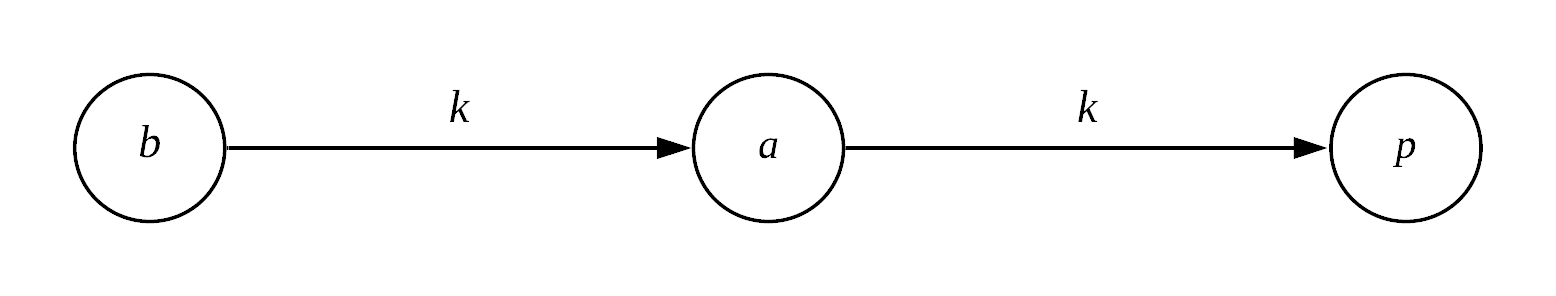
\includegraphics[scale=0.2]{images/shex-lite-rdf-graph.png}
\centering
\caption[RDF Example graph]{RDF graph formed by triplets from \cref{fig:rdf-ntriples-graph}, where
\textit{b} corresponds to \textit{\texttt{<http://example/bob>}}, \textit{a} corresponds to
\textit{\texttt{<http://example/alice>}}, \textit{p} corresponds to \textit{\texttt{<http://example/peter>}}
and \textit{k} corresponds to \textit{\texttt{<http://example/knows>}}.}
\label{fig:rdf-graph}
\end{figure}

% S E C T I O N   V A L I D A T I N G   R D F

\section{Validating RDF}
RDF therefore allows to represent and store data, and with this ability emerges the need to validate
that the schema of the graph is correct. In order to perform the validation of RDF data there  have
been previous attempts, described in \cref{sec:aaa}, this dissertation will focus
on Shape Expressions. But in order to validate RDF data every technology will need to face the following
RDF concepts:

\begin{itemize}
 \item the form of a node (the mechanisms for doing this will be called “node constraints”);
 \item the number of possible arcs incoming/outgoing from a node; and
 \item the possible values associated with those arcs.
\end{itemize}

\begin{figure}
  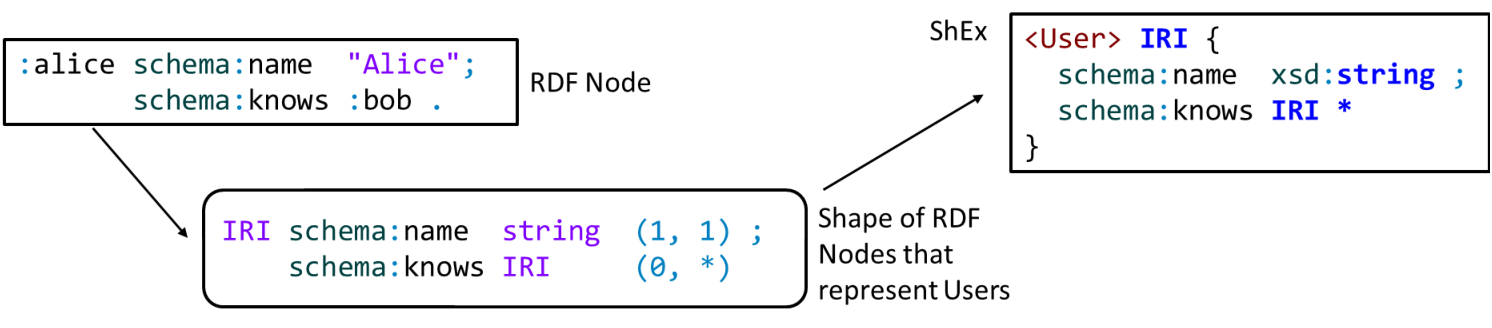
\includegraphics[scale=0.25]{images/rdf-node-and-shape.png}
  \centering
  \caption[RDF node and its shape]{RDF node and its shape.}
  \label{fig:rdf-graph-2}
\end{figure}

\cref{fig:rdf-graph} illustrates those RDF concepts by means of the Shape Expression that validates users.
There we can see that the shape of the RDF node that represents Users represents the form of a node,
the number of possible arcs and the possible value associated with those arcs.

\subsection{Shape Expressions}
As defined in \cite{labra-validating-rdf} Shape Expressions (ShEx) is a schema language for describing RDF
graphs structures. ShEx was originally developed in late 2013 to provide a human-readable syntax for OSLC
Resource Shapes. It added disjunctions, so it was more expressive than Resource Shapes. Tokens in the language
were adopted from Turtle and SPARQL with tokens for grouping, repetition and wildcards from regular expression
and RelaxNG Compact Syntax \cite{van2003relax}. The language was described in a paper
\cite{eric-rdf-validation-lang} and codified in a June 2014 W3C member submission which included a primer and
a semantics specification. This was later deemed “ShEx 1.0”.

As of publication, the ShEx Community Group was starting work on ShEx 2.1 to add features like value comparison
and unique keys. See the ShEx Homepage \url{http://shex.io/} for the state of the art in ShEx. A collection of
ShEx schemas has also been started at \url{https://github.com/shexSpec/schemas}.

\begin{figure}
\begin{lstlisting}[numbers=left, basicstyle=\ttfamily\scriptsize]
PREFIX :       <http://example.org/>
PREFIX schema: <http://schema.org/>
PREFIX xsd:  <http://www.w3.org/2001/XMLSchema#>

:User {
  schema:name          xsd:string  ;
  schema:birthDate     xsd:date?  ;
  schema:gender        [ schema:Male schema:Female ] OR xsd:string ;
  schema:knows         IRI @:User*
}
\end{lstlisting}
\caption[Shape Expression Example]{Shape Expression Example. This example describes a shape expression that
describes a user as a node that has one name of type string, an optional bithd date of type date, one gende
of type Male, Female or free string and a set between 0 and infinite of other users represented by the knows
property.}
\label{fig:shape-expr-ex}
\end{figure}

\subsubsection{ShEx Compact Syntax: \texttt{ShExC}}
The ShEx compact syntax (ShExC) was designed to be read and edited by humans. It follows some conventions which
are similar to Turtle or SPARQL.

\begin{itemize}
    \item \texttt{PREFIX} and \texttt{BASE} declarations follow the same convention as in Turtle. In the rest of
    this chapter we will omit prefix declarations for brevity.
	\item Comments start with a \texttt{\#} and continue until the end of line.
	\item The keyword a identifies the \texttt{rdf:type} property.
    \item Relative and absolute IRIs are enclosed by \texttt{< >} and prefixed names (a shorter way to write
    out IRIs) are written with prefix followed by a colon.
	\item Blank nodes are identified using \texttt{\_:label} notation.
    \item Literals can be enclosed by the same quotation conventions ( \texttt{'}, \texttt{"}, \texttt{'''},
    \texttt{"""}) as in Turtle.
    \item Keywords (apart from a) are not case sensitive. Which means that \texttt{MinInclusive} is the same
    as \texttt{MININCLUSIVE}.
\end{itemize}

A ShExC document declares a ShEx schema. A ShEx schema is a set of labeled shape expressions which are composed
of node constraints and shapes. These constrain the permissible values or graph structure around a node in an RDF
graph. When we are considering a specific node, we call that node the focus node.

\begin{figure}
  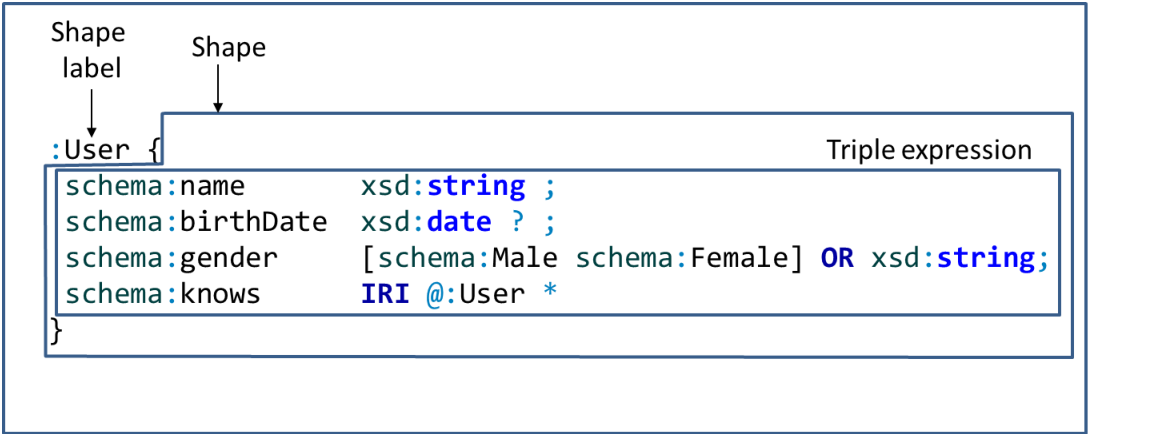
\includegraphics[scale=0.25]{images/shex-out.png}
  \centering
  \caption[Shapes, shape expression labels and triple expressions]{Shapes, shape expression labels and triple expressions.}
  \label{fig:shex-out-view}
\end{figure}

\cref{fig:shex-out-view} shows the first level of a shape expression, we have a label and the shape itself that is
what we asing to the \texttt{:User} label. Then, the shape is composed by triple expressions. The triple expression
structure is explained in \cref{fig:shex-triple-expression}, and as its name indicates it is composed of three
elements, the property, the node constraint and the cardinality.

\begin{figure}
  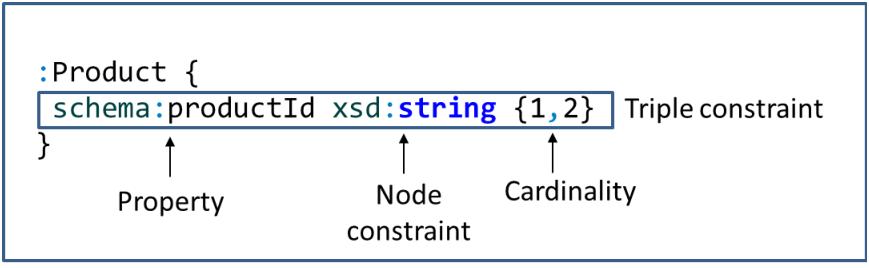
\includegraphics[scale=0.25]{images/shex-triple-expression.png}
  \centering
  \caption[Parts of a triple expression]{Parts of a triple expression.}
  \label{shex-triple-expression}
\end{figure}

Shape Expressions Compact Syntax is much bigger and containts other multiple features that give ShEx its power,
and all of them can be explored in \cite{labra-validating-rdf} but they are not needed to understand this
dissertation.

\subsubsection{Use of ShEx}
Strictly speaking, a ShEx schema defines a set of graphs. This can be used for many purposes, including
communicating data structures associated with some process or interface, generating or validating data,
or driving user interface generation and navigation. At the core of all of these use cases is the notion
of conformance with schema. Even one is using ShEx to create forms, the goal is to accept and present
data which is valid with respect to a schema. ShEx has several serialization formats:

\begin{itemize}
	\item a concise, human-readable compact syntax (ShExC);
	\item a JSON-LD syntax (ShExJ) which serves as an abstract syntax; and
	\item an RDF representation (ShExR) derived from the JSON-LD syntax.
\end{itemize}

These are all isomorphic and most implementations can map from one to another.
Tools that derive schemas by inspection or translate them from other schema languages typically generate ShExJ.
Interactions with users, e.g., in specifications are almost always in the compact syntax ShExC. As a practical
example, in HL7 FHIR, ShExJ schemas are automatically generated from other formats, and presented to the end
user using compact syntax.

ShExR allows to use RDF tools to manage schemas, e.g., doing a SPARQL query to find out whether an organization
is using dc:creator with a string, a foaf:Person, or even whether an organization is consistent about it.

\subsubsection{ShEx Implementations} \todo{Check links.}
At the time of this writing, we are aware of the following implementations of ShEx.

\begin{itemize}
	\item shex.js for Javascript/N3.js (Eric Prud’hommeaux) \url{https://github.com/shexSpec/shex.js/};
	\item Shaclex for Scala/Jena (Jose Emilio Labra Gayo) \url{https://github.com/labra/shaclex/};
	\item shex.rb for Ruby/RDF.rb (Gregg Kellogg) \url{https://github.com/ruby-rdf/shex};
	\item Java ShEx for Java/Jena (Iovka Boneva/University of Lille) \url{https://gforge.inria.fr/projects/shex-impl/}; and
	\item ShExkell for Haskell (Sergio Iván Franco and Weso Research Group) \url{https://github.com/weso/shexkell}.
\end{itemize}

There are also several online demos and tools that can be used to experiment with ShEx.

\begin{itemize}
	\item shex.js (http://rawgit.com/shexSpec/shex.js/master/doc/shex-simple.html);
	\item Shaclex (http://shaclex.herokuapp.com); and
	\item ShExValidata (for ShEx 1.0) (https://www.w3.org/2015/03/ShExValidata/).
\end{itemize}

\subsection{Other Technologies}
\label{subs:theo-back-validating-other-techs}
As other validation technologies we will just explore the existence of them as it is very interesting to know how
other tools approach the same issue.

\subsubsection{SHACL}
Also in \cite{labra-validating-rdf}, Chapter 5, it is fully explained that Shapes Constraint Language (SHACL)
has been developed by the W3C RDF Data Shapes Working Group, which was chartered in 2014 with the goal to “produce
a language for defining structural constraints on RDF graphs \cite{oslc-resource-shape}.”

The main difference that made us choose ShEx over SHACL are that ShEx emphasized human readability, with a
compact grammar that follows traditional language design principles and a compact syntax evolved from Turtle.

\subsubsection{JSON Schema}
JSON Schema born as a way to validate JSON-LD, and as turtle and RDF can be serialized as JSON-LD it is usual to
think that JSON Schema can validate RDF data, but this is not fully correct. And the reason is that the serialization
of RDF data in to JSON-LD is not deterministic, that means that a single schema might have multiple serializations,
which interferes with the validation as you cannot define a relative schema.

% S E C T I O N   P R O G R A M M I N G   L A N G U A G E S

\section{Programming Languages}
According to \cite{programing-language} “a programming language is a formal language comprising a set of instructions
that produce various kinds of output.” When we talk about programming languages we need to know that they are split into
two, General Purpose Languages (GPL) and Domain Specific Languages (DSL). The main difference overtime is that, as said
in \cite{dsl}, a domain-specific language (DSL) is a computer language specialized to a particular application domain
in contrast to a general-purpose language (GPL), which is broadly applicable across domains.

In the specific case of ShEx-Lite we will be talking about a Domain Specific Language, and more deep we would classified
it as a Declarative one, that means that it is not Touring Complete \cite{touring-complete}.

% S E C T I O N   C O M P I L E R S

\section{Compilers}
A compiler is a computer program that translates computer code written in one programming language (the source language)
into another language (the target language). Is during this translation process where the compiler validates the syntax
and the semantics of the program, if any error is detected in the process the compiler raises an exception (understand
as a compiler event that avoids the compiler to continue its execution).

\subsection{Internal Structure}
In order to decompose the internal structure of a compiler they have been split in to the most common task they do
\cref{fig:compiler-stages}, of course this doesn’t mean that there are compilers with more or less stages, but at the
end everything can be group into any of the groups that we will explain:

\begin{figure}
  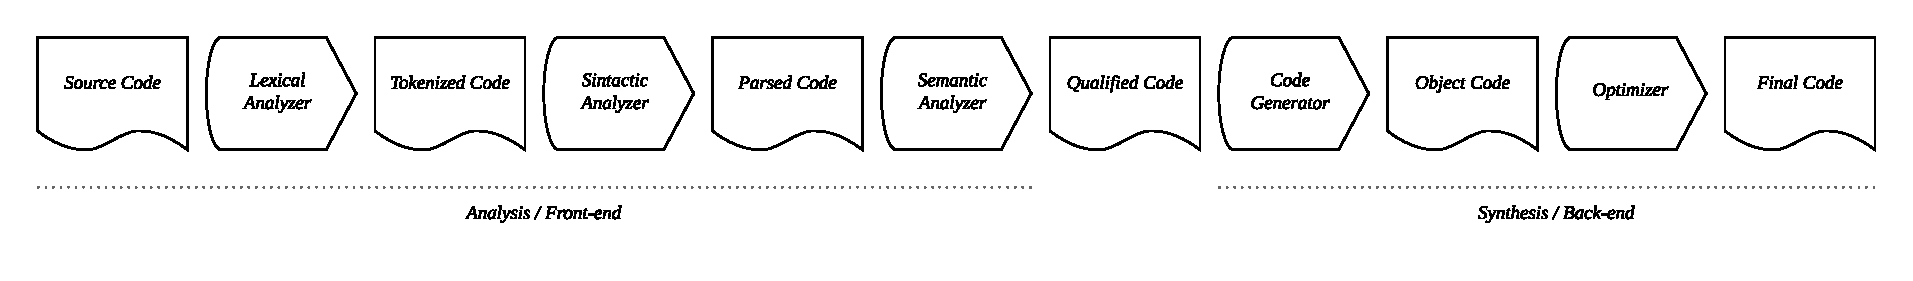
\includegraphics[width=\textwidth]{images/compiler-stages.pdf}
  \centering
  \caption[Compiler stages]{Compiler stages.}
  \label{fig:compiler-stages}
\end{figure}

\subsubsection{Lexycal Analyzer}
The lexical analyzer task is to get the input and split it in to tokens \cite{lexical-analysis}, which are build
from lexemes. If the compiler cannot find a valid token for some lexemes in the source code will generate an error,
as the input cannot be recognized.

\subsubsection{Syntactic Analyzer}
The syntactic analyzer takes the tokens generated during the lexical analysis and parses them in such a way that try’s
to group tokens so the conform to the language grammar rules. During this stage if there is any error while trying to
group the tokens then the compiler will rise an error as the input cannot be parsed.

\subsubsection{Semantic Analyzer}
The semantic analyzer has two main tasks, usually. First it validates that the source code semantics are correct, for
example 4 + “aaa” would not make sense. And the second task is to transform the Abstract Syntax Tree in to a type-checked
and annotated AST. Usually that means relate the invocations and variables to its definition, very useful for type-checking.

\subsubsection{Code Generator}
The task of the code generator as its name indicates is to generate the target code, it can be byte code, machine code
or even another high-language code.

\subsubsection{Code Optimizer}
The code optimizer is the last step before the final target code is generated, it rewrites the code that the code generator
produced without changing the semantics of the program, its aim is just to make code faster. At \cite{compiler-optimizations}
you can see an example of some optimizations that can be done at compile time to make your code faster.

\subsection{Conventional Compilers}
Conventional compiler are a big monolith where each stage \ref{fig:compiler-stages} is executed automatically after the
previous stage, if the compiler has eight steps you need to execute them all at once. This approach have been the “old-fashion”
but it presents some drawbacks:
\begin{itemize}
    \item A poor IDE \cite{ide} integration. IDE’s need to perform incremental compilations in matter of nanoseconds so
    the user doesn’t feel lag when typing the program. With conventional compilers as you need to go through all the compilation
    process at once they where very slow and companies like Microsoft need to develop different compilers, one for the IDE and
    another for the final compilation of the program itself. This lead to several problems like that if a feature gets
    implemented in the final compilation compiler but not in the IDE one the IDE would not support the feature meanwhile
    the language would.
    \item Difficult to debug. As the conventional compilers where a blackbox the only way to test intermediate stages was
    by throwing an input and waiting the the feature you wanted to test was thrown for that input.
\end{itemize}

\subsection{Modern Compilers}
After the problems Microsoft had with the C\# compiler they decide to rewrite the whole compiler and introduce a concept
called “compiler as an API” with Roslyn \cite{dotNet}. This concept has been perfectly accepted and solved many problems.
In this concept each stage has an input and an output that can be accessed from outside the compiler and stages can be
executed independently on demand. This means that for example if an IDE just want to execute the Lexer the Parser and
the Semantic analysis it can. That translates in to speed for the user.

Also the second problem is solved as testing individual parts of the compiler is much more easy than the hole compiler
at once.

\setchapterpreamble[u]{\margintoc}
\chapter{Margin Stuff}

Sidenotes are a distinctive feature of all 1.5-column-layout books. 
Indeed, having wide margins means that some material can be displayed 
there. We use margins for all kind of stuff: sidenotes, marginnotes, 
small tables of contents, citations, and, why not?, special boxes and 
environments.

\section{Sidenotes}

Sidenotes are like footnotes, except that they go in the margin, where 
they are more readable. To insert a sidenote, just use the command 
\Command{sidenote\{Text of the note\}}. You can specify a 
mark\sidenote[O]{This sidenote has a special mark, a big O!} with \\ 
\Command{sidenote[mark]\{Text\}}, but you can also specify an offset, 
which moves the sidenote upwards or downwards, so that the full syntax is:

\begin{lstlisting}[style=kaolstplain]
\sidenote[mark][offset]{Text}
\end{lstlisting}

If you use an offset, you always have to add the brackets for the mark, 
but they can be empty.\sidenote{If you want to know more about the usage 
of the \Command{sidenote} command, read the documentation of the 
\Package{sidenotes} package.}

In \Class{kaobook} we copied a feature from the \Package{snotez} 
package: the possibility to specify a multiple of \Command{baselineskip} 
as an offset. For example, if you want to enter a sidenote with the 
normal mark and move it upwards one line, type:

\begin{lstlisting}[style=kaolstplain]
\sidenote[][*-1]{Text of the sidenote.}
\end{lstlisting}

As we said, sidenotes are handled through the \Package{sidenotes} 
package, which in turn relies on the \Package{marginnote} package.

\section{Marginnotes}

This command is very similar to the previous one. You can create a 
marginnote with \Command{marginnote[offset]\{Text\}}, where the offset 
argument can be left out, or it can be a multiple of 
\Command{baselineskip},\marginnote[-1cm]{While the command for margin 
notes comes from the \Package{marginnote} package, it has been redefined 
in order to change the position of the optional offset argument, which 
now precedes the text of the note, whereas in the original version it 
was at the end. We have also added the possibility to use a multiple of 
\Command{baselineskip} as offset. These things were made only to make 
everything more consistent, so that you have to remember less things!} 
\eg

\begin{lstlisting}[style=kaolstplain]
\marginnote[-12pt]{Text} or \marginnote[*-3]{Text}
\end{lstlisting}

\begin{kaobox}[frametitle=To Do]
A small thing that needs to be done is to renew the \Command{sidenote} 
command so that it takes only one optional argument, the offset. The 
special mark argument can go somewhere else. In other words, we want the 
syntax of \Command{sidenote} to resemble that of \Command{marginnote}.
\end{kaobox}

We load the packages \Package{marginnote}, \Package{marginfix} and 
\Package{placeins}. Since \Package{sidenotes} uses \Package{marginnote}, 
what we said for marginnotes is also valid for sidenotes. Side- and 
margin- notes are shifted slightly upwards 
(\Command{renewcommand\{\textbackslash marginnotevadjust\}\{3pt\}}) in 
order to allineate them to the bottom of the line of text where the note 
is issued.

\section{Footnotes}

Even though they are not displayed in the margin, we will discuss about 
footnotes here, since sidenotes are mainly intended to be a replacement 
of them. Footnotes force the reader to constantly move from one area of 
the page to the other. Arguably, marginnotes solve this issue, so you 
should not use footnotes. Nevertheless, for completeness, we have left 
the standard command \Command{footnote}, just in case you want to put a 
footnote once in a while.\footnote{And this is how they look like. 
Notice that in the PDF file there is a back reference to the text; 
pretty cool, uh?}

\section{Margintoc}

Since we are talking about margins, we introduce here the 
\Command{margintoc} command, which allows one to put small table of 
contents in the margin. Like other commands we have discussed, 
\Command{margintoc} accepts a parameter for the vertical offset, like 
so: \Command{margintoc[offset]}.

The command can be used in any point of the document, but we think it 
makes sense to use it just at the beginning of chapters or parts. In 
this document I make use of a \KOMAScript\xspace feature and put it in 
the chapter preamble, with the following code:

\marginnote{The font used in the margintoc is the same as the one for 
	the chapter entries in the main table of contents at the beginning 
	of the document.}

\begin{lstlisting}[style=kaolstplain]
\setchapterpreamble[u]{\margintoc}
\chapter{Chapter title}
\end{lstlisting}

\section{Marginlisting}

On some occasions it may happen that you have a very short piece of code 
that doesn't look good in the body of the text because it breaks the 
flow of narration: for that occasions, you can use a 
\Environment{marginlisting}. The support for this feature is still 
limited, especially for the captions, but you can try the following 
code:

\begin{marginlisting}[-1.35cm]
	\caption{An example of a margin listing.}
	\vspace{0.6cm}
	\begin{lstlisting}[language=Python,style=kaolstplain]
print("Hello World!")
	\end{lstlisting}
\end{marginlisting}

\begin{verbatim}
\begin{marginlisting}[-0.5cm]
	\caption{My caption}
	\vspace{0.2cm}
	\begin{lstlisting}[language=Python,style=kaolstplain]
	... code ...
	\end{lstlisting}
\end{marginlisting}
\end{verbatim}

Unfortunately, the space between the caption and the listing must be 
adjusted manually; if you find a better way, please let me know.

Not only textual stuff can be displayed in the margin, but also figures. 
Those will be the focus of the next chapter.

\setchapterimage[6.5cm]{seaside}
\setchapterpreamble[u]{\margintoc}
\chapter[Figures and Tables]{Figures and Tables\footnotemark[0]}

\footnotetext{The credits for the image above the chapter title go to:
	Bushra Feroz --- Own work, CC~BY-SA~4.0, 
	\url{https://commons.wikimedia.org/w/index.php?curid=68724647}}

\section{Normal Figures and Tables}

Figures and tables can be inserted just like in any standard 
\LaTeX\xspace document. The \Package{graphicx} package is already loaded 
and configured in such a way that the figure width is equal to the 
textwidth and the height is adjusted in order to maintain the original 
aspect ratio. As you may have imagined, the captions will be 
positioned\ldots well, in the margins. This is achieved with the help of 
the \Package{floatrow} package.

Here is a picture of Mona Lisa (\reffig{normalmonalisa}), as an example. 
The captions are formatted as the margin- and the side-notes; If you 
want to change something about captions you can use the command 
\Command{captsetup} from the \Package{caption} package. Remember that if 
you want to reference a figure, the label must come \emph{after} the 
caption!

\begin{figure}[hb]
	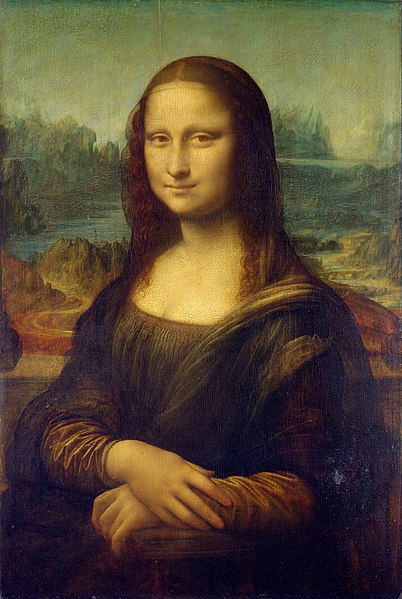
\includegraphics[width=0.45\textwidth]{monalisa}
	\caption[Mona Lisa, again]{It's Mona Lisa again. \blindtext}
	\labfig{normalmonalisa}
\end{figure}

While the format of the caption is managed by \Package{caption}, its 
position is handled by the \Package{floatrow} package. Achieving this 
result has been quite hard, but now I am pretty satisfied. In two-side 
mode, the captions are printed in the correct margin.

Tables can be inserted just as easily as figures, as exemplified by the 
following code:

\begin{lstlisting}[caption={Caption of a listing.}]
\begin{table}
\begin{tabular}{ c c c c }
	\toprule
	col1 & col2 & col3 & col 4 \\
	\midrule
	\multirow{3}{4em}{Multiple row} & cell2 & cell3 & cell4\\ &
	cell5 & cell6 & cell7 \\ &
	cell8 & cell9 & cell10 \\
	\multirow{3}{4em}{Multiple row} & cell2 & cell3 & cell4 \\ &
	cell5 & cell6 & cell7 \\ &
	cell8 & cell9 & cell10 \\
	\bottomrule
\end{tabular}
\end{table}
\end{lstlisting}

which results in the useless \vreftab{useless}.

\begin{table}[h]
\caption[A useless table]{A useless table.}
\labtab{useless}
\begin{tabular}{ c c c c }
	\toprule
	col1 & col2 & col3 & col 4 \\
	\midrule
	\multirow{3}{4em}{Multiple row} & cell2 & cell3 & cell4\\ &
	cell5 & cell6 & cell7 \\ &
	cell8 & cell9 & cell10 \\
	\multirow{3}{4em}{Multiple row} & cell2 & cell3 & cell4 \\ &
	cell5 & cell6 & cell7 \\ &
	cell8 & cell9 & cell10 \\
	\bottomrule
\end{tabular}
\end{table}

I don't have much else to say, so I will just insert some blind text. 
\blindtext

\section{Margin Figures and Tables}

Marginfigures can be inserted with the environment 
\Environment{marginfigure}. In this case, the whole picture is confined 
to the margin and the caption is below it. \reffig{marginmonalisa} is 
obtained with something like this:

\begin{lstlisting}[caption={Another caption.}]
\begin{marginfigure}
	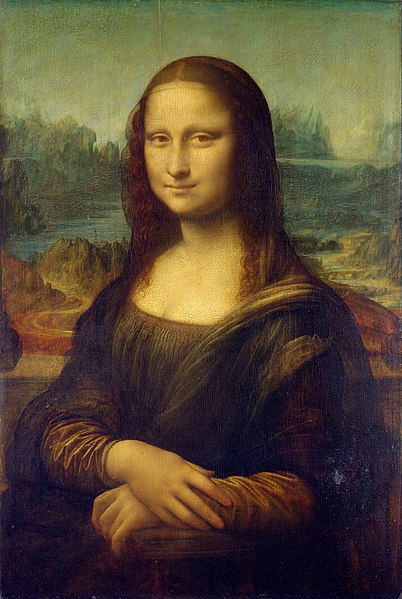
\includegraphics{monalisa}
	\caption[The Mona Lisa]{The Mona Lisa.}
	\labfig{marginmonalisa}
\end{marginfigure}
\end{lstlisting}

There is also the \Environment{margintable} environment, of which 
\reftab{anotheruseless} is an example. Notice how you can place the 
caption above the table by just placing the \Command{caption} command 
before beginning the \Environment{tabular} environment. Usually, figure 
captions are below, while table captions are above. This rule is also 
respected for normal figures and tables: the captions are always on the 
side, but for figure they are aligned to the bottom, while for tables to 
the top.

\begin{margintable}
\caption[Another useless table]{Another useless table.}
\labtab{anotheruseless}
\raggedright
\begin{tabular}{ c c c c }
	\hline
	col1 & col2 & col3 \\
	\hline
	\multirow{3}{4em}{Multiple row} & cell2 & cell3 \\ & cell5 & cell6 
	\\ & cell8 & cell9 \\ \hline
\end{tabular}
\end{margintable}

Marginfigures and tables can be positioned with an optional offset 
command, like so:

\begin{lstlisting}
\begin{marginfigure}[offset]
	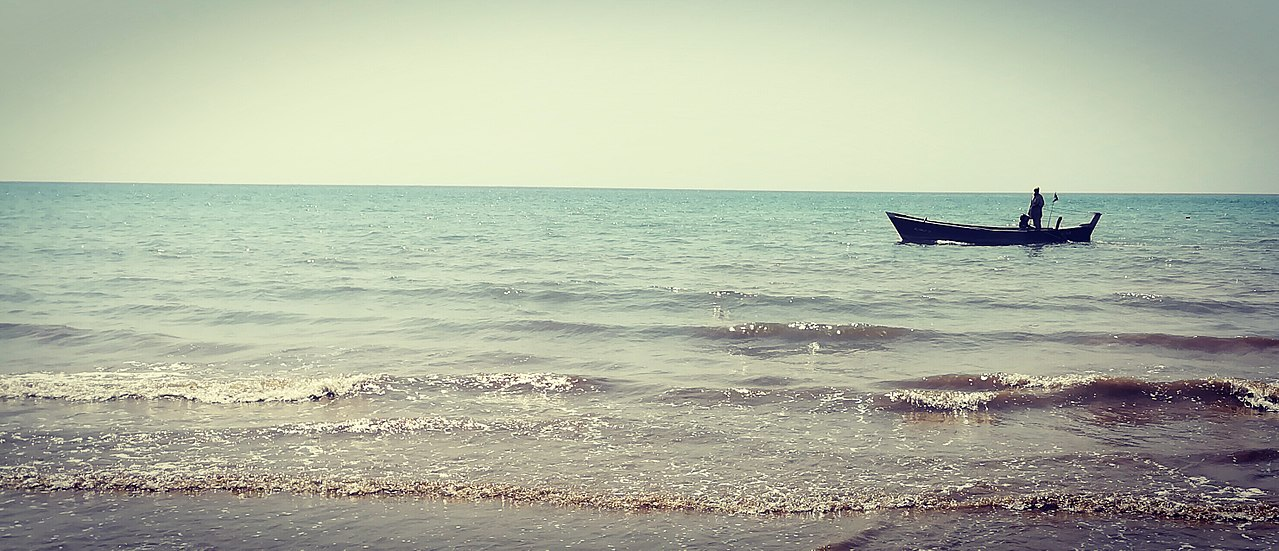
\includegraphics{seaside}
\end{marginfigure}
\end{lstlisting}

Offset ca be either a measure or a multiple of \Command{baselineskip}, 
much like with \Command{sidenote}, \Command{marginnote} and 
\Command{margintoc}.\todo{Improve this part.} If you are wondering how I 
inserted this orange bubble, have a look at the \Package{todo} package.

\section{Wide Figures and Tables}

\begin{figure*}[h!]
	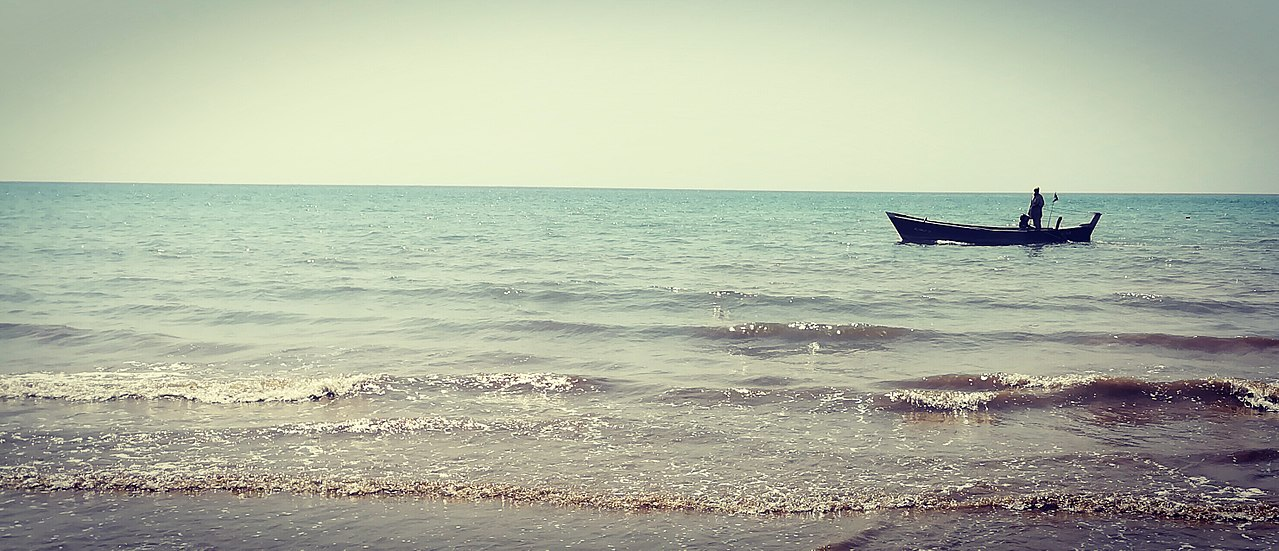
\includegraphics{seaside}
	\caption[A wide seaside]{A wide seaside, and a wide caption.
		Credits: By Bushra Feroz --- Own work, CC BY-SA 4.0, 
		\url{https://commons.wikimedia.org/w/index.php?curid=68724647}}
\end{figure*}

With the environments \Environment{figure*} and \Environment{table*} you 
can insert figures which span the whole page width. The caption will be 
positioned below or above, according to taste.

You may have noticed the full width image at the very beginning of this 
chapter: that, however, is set up in an entirely different way, which 
you'll read about in \vrefch{layout}. Now it is time to tackle 
hyperreferences.

\setchapterstyle{kao}
%\setchapterpreamble[u]{\margintoc}
\chapter{References}
\labch{references}

\section{Citations}

\index{citations}
To cite someone \sidecite{Visscher2008,James2013} is very simple: just 
use the \Command{sidecite}\index{\Command{sidecite}} command. It does 
not have an offset argument yet, but it probably will in the future. 
This command supports multiple entries, as you can see, and by default 
it prints the reference on the margin as well as adding it to the 
bibliography at the end of the document. Note that the citations have 
nothing to do with the text,\sidecite{James2013} but they are completely 
random as they only serve the purpose to illustrate the feature.

For this setup I wrote a separate package, \Package{kaobiblio}, which 
you can find in the \Package{styles} directory and include in your main 
tex file. This package accepts all the options that you can pass to 
\Package{biblatex}, and actually it passes them to \Package{biblatex} 
under the hood. Moreover, it also defines some commands, like 
\Command{sidecite}, and environments that can be used within a 
\Class{kao} book.\sidenote{For this reason you should always use 
\Package{kaobiblio} instead of \Package{biblatex}, but the syntax and 
the options are exactly the same.}

As you have seen, the \Command{sidecite} command will print a citation 
in the margin. However, this command would be useless without a way to 
customise the format of the citation, so the \Class{kaobook} provides 
also the \Command{formatmargincitation} command. By \enquote{renewing} 
that command, you can choose which items will be printed in the margins. 
The best way to understand how it works is to see the actual definition 
of this command.

\begin{lstlisting}[style=kaolstplain,linewidth=1.5\textwidth]
\newcommand{\formatmargincitation}[1]{
	\parencite{#1}: \citeauthor*{#1} (\citeyear{#1}), \citetitle{#1}\\
}
\end{lstlisting}

Thus, the \Command{formatmargincitation} accepts one parameter, which is 
the citation key, and prints the parencite followed by a colon, then the 
author, then the year (in brackets), and finally the 
title.\sidecite{Battle2014} Now, suppose that you wish the margin 
citation to display the year and the author, followed by the title, and 
finally a fixed arbitrary string; you would add to your document:

\begin{lstlisting}[style=kaolstplain,linewidth=1.5\textwidth]
\renewcommand{\formatmargincitation}[1]{
	\citeyear{#1}, \citeauthor*{#1}: \citetitle{#1}; very interesting!\\
}
\end{lstlisting}

\renewcommand{\formatmargincitation}[1]{
	\citeyear{#1}, \citeauthor*{#1}: \citetitle{#1}; very interesting!\\
}

The above code results in citations that look like the 
following.\sidecite{Zou2005} Of course, changing the format is most 
useful when you also change the default bibliography style. For 
instance, if you want to use the \enquote{philosophy-modern} style for 
your bibliography, you might have something like this in the preamble:

\begin{lstlisting}[style=kaolstplain,linewidth=1.5\textwidth]
\usepackage[style=philosophy-modern]{styles/kaobiblio}
\renewcommand{\formatmargincitation}[1]{
	\sdcite{#1}\\
}
\addbibresource{main.bib}
\end{lstlisting}

\renewcommand{\formatmargincitation}[1]{
	\parencite{#1}: \citeauthor*{#1} (\citeyear{#1}), \citetitle{#1}\\
}

The commands like \Command{citeyear}, \Command{parencite} and 
\Command{sdcite} are just examples. A full reference of the available 
commands can be found in this 
\href{http://tug.ctan.org/info/biblatex-cheatsheet/biblatex-cheatsheet.pdf}{cheatsheet}, 
under the \enquote{Citations} section.

Finally, to compile a document containing citations, you need to use an 
external tool, which for this class is biber. You need to run the 
following (assuming that your tex file is called main.tex):

\begin{lstlisting}[style=kaolstplain]
$ pdflatex main
$ biber main
$ pdflatex main
\end{lstlisting}

\section{Glossaries and Indices}

\index{glossary}
The \Class{kaobook} class loads the packages \Package{glossaries} and 
\Package{imakeidx}, with which you can add glossaries and indices to 
your book. For instance, I previously defined some glossary entries and 
now I am going to use them, like this: \gls{computer}. 
\Package{glossaries} also allows you to use acronyms, like the 
following: this is the full version, \acrfull{fpsLabel}, and this is the 
short one \acrshort{fpsLabel}. These entries will appear in the glossary 
in the backmatter.

Unless you use \href{https://www.overleaf.com}{Overleaf} or some other 
fancy IDE for \LaTeX, you need to run an external command from your 
terminal in order to compile a document with a glossary. In particular, 
the commands required are:\sidenote{These are the commands you 
would run in a UNIX system; I have no idea on how it works in Windows.}

\begin{lstlisting}[style=kaolstplain]
$ pdflatex main
$ makeglossaries main
$ pdflatex main
\end{lstlisting}

Note that you need not run \texttt{makeglossaries} every time you 
compile your document, but only when you change the glossary entries.

\index{index}
To create an index, you need to insert the command 
\lstinline|\index{subject}| whenever you are talking about 
\enquote{subject} in the text. For instance, at the start of this 
paragraph I would write \lstinline|index{index}|, and an entry would be 
added to the Index in the backmatter. Check it out!

\marginnote[2mm]{In theory, you would need to run an external command 
for the index as well, but luckily the package we suggested, 
	\Package{imakeidx}, can compile the index automatically.}

\index{nomenclature}
A nomenclature is just a special kind of index; you can find one at the end of
this book. To insert a nomenclature, we use the package \Package{nomencl} and
add the terms with the command \Command{nomenclature}. We put then a
\Command{printnomenclature} where we want it to appear.

Also with this package we need to run an external command to compile the 
document, otherwise the nomenclature will not appear:

\begin{lstlisting}[style=kaolstplain]
$ pdflatex main
$ makeindex main.nlo -s nomencl.ist -o main.nls
$ pdflatex main
\end{lstlisting}

These packages are all loaded in 
\href{style/packages.sty}{packages.sty}, one of the files that come with 
this class. However, the configuration of the elements is best done in 
the main.tex file, since each book will have different entries and 
styles.

Note that the \Package{nomencl} package caused problems when the 
document was compiled, so, to make a long story short, I had to prevent 
\Package{scrhack} to load the hack-file for \Package{nomencl}. When 
compiling the document on Overleaf, however, this problem seem to 
vanish.

\marginnote[-19mm]{This brief section was by no means a complete 
reference on the subject, therefore you should consult the documentation 
of the above package to gain a full understanding of how they work.}

\section{Hyperreferences}
\labsec{hyprefs}

\index{hyperreferences}
In this class we provide a handy sub-package to help you referencing the 
same elements always in the same way, for consistency across the book. 
First, you can label each element with a specific command. For instance, 
should you want to label a chapter, you would put 
\lstinline|\labch{chapter-title}| right after the \Command{chapter} 
directive. This is just a convienence, because \Command{labch} is 
actually just an alias to \lstinline|\label{ch:chapter-title}|, so it 
spares you the writing of \enquote{ch}. We defined similar commands for 
many typically labeled elements, including:

\begin{multicols}{2}
\setlength{\columnseprule}{0pt}
\begin{itemize}
	\item Page: \Command{labpage}
	\item Part: \Command{labpart}
	\item Chapter: \Command{labch}
	\item Section: \Command{labsec}
	\item Figure: \Command{labfig}
	\item Table: \Command{labtab}
	\item Definition: \Command{labdef}
	\item Theorem: \Command{labthm}
	\item Proposition: \Command{labprop}
	\item Lemma: \Command{lablemma}
	\item Remark: \Command{labremark}
	\item Example: \Command{labexample}
	\item Exercise: \Command{labexercise}
\end{itemize}
\end{multicols}

Of course, we have similar commands for referencing those elements. 
However, since the style of the reference should depend on the context, 
we provide different commands to reference the same thing. For instance, 
in some occasions you may want to reference the chapter by name, but 
other times you want to reference it only by number. In general, there 
are four reference style, which we call plain, vario, name, and full. 

The plain style references only by number. It is accessed, for chapters, 
with \lstinline|\refch{chapter-title}| (for other elements, the syntax 
is analogous). Such a reference results in: \refch{references}.

The vario and name styles rest upon the \Package{varioref} package. 
Their syntax is \lstinline|\vrefch{chapter-title}| and 
\lstinline|\nrefch{chapter-title}|, and they result in: 
\vrefch{references}, for the vario style, and: \nrefch{references}, for 
the name style. As you can see, the page is referenced in 
\Package{varioref} style.

The full style references everything. You can use it with 
\lstinline|\frefch{chapter-title}| and it looks like this: 
\frefch{references}.

Of course, all the other elements have similar commands (\eg for parts 
you would use \lstinline|\vrefpart{part-title}| or something like that). 
However, not all elements implement all the four styles. The commands 
provided should be enough, but if you want to see what is available or 
to add the missing ones, have a look at the 
\href{styles/kaorefs.sty}{attached package}.


\pagelayout{wide} % No margins
\addpart{Design and Additional Features}
\pagelayout{margin} % Restore margins

\setchapterimage[6cm]{seaside}
\setchapterpreamble[u]{\margintoc}
\chapter{Page Design}
\labch{layout}

\section{Headings}

So far, in this document I used two different styles for the chapter 
headings: one has the chapter name, a rule and, in the margin, the 
chapter number; the other has an image at the top of the page, and the 
chapter title is printed in a box (like for this chapter). There is one 
additional style, which I used only in the appendix 
(\vrefpage{appendix}); there, the chapter title is enclosed in two 
horizontal rules, and the chapter number (or letter, in the case of the 
appendix) is above it.\sidenote{To be honest, I do not think that mixing 
heading styles like this is a wise choice, but in this document I did it 
only to show you how they look.}

Every book is unique, so it makes sense to have different styles from 
which to choose. Actually, it would be awesome if whenever a 
\Class{kao}-user designs a new heading style, he or she added it to the 
three styles already present, so that it will be available for new users 
and new books.

The choice of the style is made simple by the \Command{setchapterstyle} 
command. It accepts one option, the name of the style, which can be: 
\enquote{plain}, \enquote{kao}, or \enquote{lines}.\sidenote{Plain is 
the default \LaTeX\xspace title style; the other ones are self 
explanatory.} If instead you want the image style, you have to use the 
command \Command{setchapterimage}, which accepts the path to the image 
as argument; you can also provide an optional parameter in square 
brackets to specify the height of the image.

Let us make some examples. In this book, I begin a normal chapter with 
the lines:

\begin{lstlisting}
\setchapterstyle{kao}
\setchapterpreamble[u]{\margintoc}
\chapter{Title of the Chapter}
\labch{title}
\end{lstlisting}

In Line 1 I choose the style for the title to be \enquote{kao}. Then, I 
specify that I want the margin toc. The rest is ordinary administration 
in \LaTeX, except that I use my own \Command{labch} to label the 
chapter. Actually, the \Command{setchapterpreamble} is a standard 
\KOMAScript\xspace one, so I invide you to read about it in the KOMA 
documentation. Once the chapter style is set, it holds until you change 
it.\sidenote{The \Command{margintoc} has to be specified at every 
chapter. Perhaps in the future this may change; it all depends on how 
this feature will be welcomed by the users, so keep in touch with me if 
you have preferences!} Whenever I want to start a chapter with an image, 
I simply write:

\begin{lstlisting}
\setchapterimage[7cm]{path/to/image.png} % Optionally specify the height
\setchapterpreamble[u]{\margintoc}
\chapter{Catchy Title} % No need to set a chapter style
\labch{catchy}
\end{lstlisting}

If you prefer, you can also specify the style at the beginning of the 
main document, and that style will hold until you change it again.

\section{Headers \& Footers}

Headers and footers in \KOMAScript\xspace are handled by the 
\Package{scrlayer-scrpage} package. There are two basic style: 
\enquote{scrheadings} and \enquote{plain.scrheadings}. The former is 
used for normal pages, whereas the latter is used in title pages (those 
where a new chapter starts, for instance) and, at least in this book, in 
the front matter. At any rate, the style can be changed with the 
\Command{pagestyle} command, \eg 
\lstinline|\pagestyle{plain.scrheadings}|.

In both stles, the footer is completely empty. In plain.scrheadings, 
also the header is absent (otherwise it wouldn't be so plain\ldots), but 
in the normal style the design is reminescent of the \enquote{kao} style 
for chapter titles.

\begin{kaobox}[frametitle=To Do]
The \Option{twoside} class option is still unstable and may lead to 
unexpected behaviours. As always, any help will be greatly appreciated.
\end{kaobox}

\section{Table of Contents}

Another important part of a book is the table of contents. By default, 
in \Class{kaobook} there is an entry for everything: list of figures, 
list of tables, bibliographies, and even the table of contents itself. 
Not everybody might like this, so we will provide a description of the 
changes you need to do in order to enable or disable each of these 
entries. In the following \reftab{tocentries}, each item corresponds to 
a possible entry in the \acrshort{tocLabel}, and its description is the 
command you need to provide to have such entry. These commands are 
specified in the attached \href{style/style.sty}{style 
package},\sidenote{In the same file, you can also choose the titles of 
these entries.} so if you don't want the entries, just comment the 
corresponding lines.

Of course, some packages, like those for glossaries and indices, will 
try to add their own entries.\marginnote{In a later section, we will see 
how you can define your own floating environment, and endow it with an 
entry in the \acrshort{tocLabel}.} In such cases, you have to follow the 
instructions specific to that package. Here, since we have talked about 
glossaries and notations in \refch{references}, we will biefly see how 
to configure them.

\begin{table}
\footnotesize
\caption{Commands to add a particular entry to the table of contents.}
\labtab{tocentries}
\begin{tabular}{ l l }
	\toprule
	Entry & Command to Activate \\
	\midrule
	Table of Contents & \lstinline|\setuptoc{toc}{totoc}| \\
	List of Figs and Tabs & \lstinline|\PassOptionsToClass{toc=listof}{\@baseclass}| \\
	Bibliography & \lstinline|\PassOptionsToClass{toc=bibliography}{\@baseclass}| \\
	\bottomrule
\end{tabular}
\end{table}

For the \Package{glossaries} package, use the \enquote{toc} option when 
you load it: \lstinline|\usepackage[toc]{glossaries}|. For 
\Package{nomencl}, pass the \enquote{intoc} option at the moment of 
loading the package. Both \Package{glossaries} and \Package{nomencl} are 
loaded in the attached \href{style/packages.sty}{\enquote{packages} 
package}.

Additional configuration of the table of contents can be performed 
through the packages \Package{etoc}, which is loaded because it is 
needed for the margintocs, or the more traditional \Package{tocbase}. 
Read the respective documentations if you want to be able to change the 
default \acrshort{tocLabel} style.\sidenote[][*-1]{(And please, send me 
a copy of what you have done, I'm so curious!)}

\section{Page Layout}

Besides the page style, you can also change the width of the content of 
a page. This is particularly useful for pages dedicated to part titles, 
where having the 1.5-column layout might be a little awkward, or for 
pages where you only put figures, where it is important to exploit all 
the available space.

In practice, there are two layouts: \enquote{wide} and \enquote{margin}. 
The former suppresses the margins and allocates the full page for 
contents, while the latter is the layout used in most of the pages of 
this book, including this one. The wide layout is also used 
automatically in the front and back matters.

To change page layout, use the \Command{pagelayout} command. For 
example, when I start a new part, I write:

\begin{lstlisting}
\pagelayout{wide}
\addpart{Title of the New Part}
\pagelayout{margin}
\end{lstlisting}

\section{Numbers \& Counters}

In this short section we shall see how dispositions, sidenotes and 
figures are numbered in the \Class{kaobook} class.

By default, dispositions are numbered up to the section. This is 
achieved by setting: \lstinline|\setcounter{secnumdepth}{1}|.

The sidenotes counter is the same across all the document, but if you 
want it to reset at each chapter, just uncomment the line

\begin{lstlisting}[style=kaolstplain]
\counterwithin*{sidenote}{chapter}
\end{lstlisting}

in the \Package{styles/style.sty} package provided by this class.

Figure and Table numbering is also per-chapter; to change that, use 
something like:

\begin{lstlisting}[style=kaolstplain]
\renewcommand{\thefigure}{\arabic{section}.\arabic{figure}}
\end{lstlisting}

\section{White Space}

One of the things that I find most hard in \LaTeX\xspace is to finely 
tune the white space around objects. There are not fixed rules, each 
object needs its own adjustment. Here we shall see how some spaces are 
defined at the moment in this class.\marginnote{Attention! This section 
may be incomplete.}

\textbf{Space around figures and tables}

\begin{lstlisting}[style=kaolstplain]
\renewcommand\FBaskip{.4\topskip}
\renewcommand\FBbskip{\FBaskip}
\end{lstlisting}

\textbf{Space around captions}

\begin{lstlisting}[style=kaolstplain]
\captionsetup{
	aboveskip=6pt,
	belowskip=6pt
}
\end{lstlisting}

\textbf{Space around displays (\eg equations)}

\begin{lstlisting}[style=kaolstplain]
\setlength\abovedisplayskip{6pt plus 2pt minus 4pt}
\setlength\belowdisplayskip{6pt plus 2pt minus 4pt}
\abovedisplayskip 10\p@ \@plus2\p@ \@minus5\p@
\abovedisplayshortskip \z@ \@plus3\p@
\belowdisplayskip \abovedisplayskip
\belowdisplayshortskip 6\p@ \@plus3\p@ \@minus3\p@
\end{lstlisting}

\setchapterstyle{kao}
\setchapterpreamble[u]{\margintoc}
\chapter{Mathematics and Boxes}
\labch{mathematics}

\section{Theorems}

Despite most people complain at the sight of a book full of equations, 
mathematics is an important part of many books. Here, we shall 
illustrate some of the possibilities. We believe that theorems, 
definitions, remarks and examples should be emphasised with a shaded 
background; however, the colour should not be to heavy on the eyes, so 
we have chosen a sort of light yellow.\sidenote{The boxes are all of the 
same colour here, because we did not want our document to look like 
\href{https://en.wikipedia.org/wiki/Harlequin}{Harlequin}.}

\begin{definition}
\labdef{openset}
Let $(X, d)$ be a metric space. A subset $U \subset X$ is an open set 
if, for any $x \in U$ there exists $r > 0$ such that $B(x, r) \subset 
U$. We call the topology associated to d the set $\tau\textsubscript{d}$ 
of all the open subsets of $(X, d).$
\end{definition}

\refdef{openset} is very important. I am not joking, but I have inserted 
this phrase only to show how to reference definitions. The following 
statement is repeated over and over in different environments.

\begin{theorem}
A finite intersection of open sets of (X, d) is an open set of (X, d), 
i.e $\tau\textsubscript{d}$ is closed under finite intersections. Any 
union of open sets of (X, d) is an open set of (X, d).
\end{theorem}

\begin{proposition}
A finite intersection of open sets of (X, d) is an open set of (X, d), 
i.e $\tau\textsubscript{d}$ is closed under finite intersections. Any 
union of open sets of (X, d) is an open set of (X, d).\marginnote{You can even insert footnotes inside the theorem 
	environments; they will be displayed at the bottom of the box.}
\end{proposition}

\begin{lemma}
A finite intersection\footnote{I'm a footnote} of open sets of (X, d) is 
an open set of (X, d), i.e $\tau\textsubscript{d}$ is closed under 
finite intersections. Any union of open sets of (X, d) is an open set of 
(X, d).
\end{lemma}

You can safely ignore the content of the theorems\ldots I assume that if 
you are interested in having theorems in your book, you already know 
something about the classical way to add them. These example should just 
showcase all the things you can do within this class.

\begin{corollary}[Finite Intersection, Countable Union]
A finite intersection of open sets of (X, d) is an open set of (X, d), 
i.e $\tau\textsubscript{d}$ is closed under finite intersections. Any 
union of open sets of (X, d) is an open set of (X, d).
\end{corollary}

\begin{proof}
The proof is left to the reader as a trivial exercise. Hint: \blindtext
\end{proof}

\begin{definition}
Let $(X, d)$ be a metric space. A subset $U \subset X$ is an open set 
if, for any $x \in U$ there exists $r > 0$ such that $B(x, r) \subset 
U$. We call the topology associated to d the set $\tau\textsubscript{d}$ 
of all the open subsets of $(X, d).$\marginnote{
	Here is a random equation, just because we can:
	\begin{equation*}
  x = a_0 + \cfrac{1}{a_1
          + \cfrac{1}{a_2
          + \cfrac{1}{a_3 + \cfrac{1}{a_4} } } }
	\end{equation*}
}
\end{definition}

\begin{example}
Let $(X, d)$ be a metric space. A subset $U \subset X$ is an open set 
if, for any $x \in U$ there exists $r > 0$ such that $B(x, r) \subset 
U$. We call the topology associated to d the set $\tau\textsubscript{d}$ 
of all the open subsets of $(X, d).$
\end{example}

\begin{remark}
Let $(X, d)$ be a metric space. A subset $U \subset X$ is an open set 
if, for any $x \in U$ there exists $r > 0$ such that $B(x, r) \subset 
U$. We call the topology associated to d the set $\tau\textsubscript{d}$ 
of all the open subsets of $(X, d).$
\end{remark}

As you may have noticed, definitions, example and remarks have 
independent counters; theorems, propositions, lemmas and corollaries 
share the same counter.

\begin{remark}
Here is how an integral looks like inline: $\int_{a}^{b} x^2 dx$, and 
here is the same integral displayed in its own paragraph:
\[\int_{a}^{b} x^2 dx\]
\end{remark}

We provide two files for the theorem styles: 
\href{style/plaintheorems.sty}{plaintheorems.sty}, which you should 
include if you do not want coloured boxes around theorems; and 
\href{style/mdftheorems.sty}{mdftheorems.sty}, which is the one used for 
this document.\sidenote{The plain one is not showed, but actually it is 
exactly the same as this one, only without the yellow boxes.} Of course, 
you will have to edit these files according to your taste and the 
general style of the book.

\section[Boxes \& Environments]{Boxes \& Custom Environments
\sidenote[][*1.8]{Notice that in the table of contents and in the 
	header, the name of this section is \enquote{Boxes \& Environments}; 
	we achieved this with the optional argument of the \texttt{section} 
	command.}}

Say you want to insert a special section, an optional content or just 
something you want to emphasise. We think that nothing works better than 
a box in these cases. We used \Package{mdframed} to construct the ones 
shown below. You can create and modify such environments by editing the 
provided file \href{style/environments.sty}{environments.sty}.

\begin{kaobox}[frametitle=Title of the box]
\blindtext
\end{kaobox}

If you set up a counter, you can even create your own numbered 
environment.

\begin{kaocounter}
	\blindtext
\end{kaocounter}

\section{Experiments}

It is possible to wrap marginnotes inside boxes, too. Audacious readers 
are encouraged to try their own experiments and let me know the 
outcomes.

\marginnote[-2.2cm]{
	\begin{kaobox}[frametitle=title of margin note]
		Margin note inside a kaobox.\\
		(Actually, kaobox inside a marginnote!)
	\end{kaobox}
}

I believe that many other special things are possible with the 
\Class{kaobook} class. During its development, I struggled to keep it as 
flexible as possible, so that new features could be added without too 
great an effort. Therefore, I hope that you can find the optimal way to 
express yourselves in writing a book, report or thesis with this class, 
and I am eager to see the outcomes of any experiment that you may try.

%\begin{margintable}
	%\captionsetup{type=table,position=above}
	%\begin{kaobox}
		%\caption{caption}
		%\begin{tabular}{ |c|c|c|c| }
			%\hline
			%col1 & col2 & col3 \\
			%\hline
			%\multirow{3}{4em}{Multiple row} & cell2 & cell3 \\ & cell5 
			%%& cell6 \\ 
			%& cell8 & cell9 \\
			%\hline
		%\end{tabular}
	%\end{kaobox}
%\end{margintable}


\appendix % From here onwards, chapters are numbered with letters, as is the appendix convention

\pagelayout{wide} % No margins
\addpart{Appendix}
\pagelayout{margin} % Restore margins

\setchapterstyle{lines}
\labpage{appendix}
\blinddocument


%----------------------------------------------------------------------------------------

\backmatter % Denotes the end of the main document content
\setchapterstyle{plain} % Output plain chapters from this point onwards

%----------------------------------------------------------------------------------------
%	BIBLIOGRAPHY
%----------------------------------------------------------------------------------------

% The bibliography needs to be compiled with biber using your LaTeX editor, or on the command line with 'biber main' from the template directory

\defbibnote{bibnote}{Here are the references in citation order.\par\bigskip} % Prepend this text to the bibliography
\printbibliography[heading=bibintoc, title=Bibliography, prenote=bibnote] % Add the bibliography heading to the ToC, set the title of the bibliography and output the bibliography note

%----------------------------------------------------------------------------------------
%	NOMENCLATURE
%----------------------------------------------------------------------------------------

% The nomenclature needs to be compiled on the command line with 'makeindex main.nlo -s nomencl.ist -o main.nls' from the template directory

\nomenclature{$c$}{Speed of light in a vacuum inertial frame}
\nomenclature{$h$}{Planck constant}

\renewcommand{\nomname}{Notation} % Rename the default 'Nomenclature'
\renewcommand{\nompreamble}{The next list describes several symbols that will be later used within the body of the document.} % Prepend this text to the nomenclature

\printnomenclature % Output the nomenclature

%----------------------------------------------------------------------------------------
%	GREEK ALPHABET
% 	Originally from https://gitlab.com/jim.hefferon/linear-algebra
%----------------------------------------------------------------------------------------

\vspace{1cm}

{\usekomafont{chapter}Greek Letters with Pronounciation} \\[2ex]
\begin{center}
	\newcommand{\pronounced}[1]{\hspace*{.2em}\small\textit{#1}}
	\begin{tabular}{l l @{\hspace*{3em}} l l}
		\toprule
		Character & Name & Character & Name \\ 
		\midrule
		$\alpha$ & alpha \pronounced{AL-fuh} & $\nu$ & nu \pronounced{NEW} \\
		$\beta$ & beta \pronounced{BAY-tuh} & $\xi$, $\Xi$ & xi \pronounced{KSIGH} \\ 
		$\gamma$, $\Gamma$ & gamma \pronounced{GAM-muh} & o & omicron \pronounced{OM-uh-CRON} \\
		$\delta$, $\Delta$ & delta \pronounced{DEL-tuh} & $\pi$, $\Pi$ & pi \pronounced{PIE} \\
		$\epsilon$ & epsilon \pronounced{EP-suh-lon} & $\rho$ & rho \pronounced{ROW} \\
		$\zeta$ & zeta \pronounced{ZAY-tuh} & $\sigma$, $\Sigma$ & sigma \pronounced{SIG-muh} \\
		$\eta$ & eta \pronounced{AY-tuh} & $\tau$ & tau \pronounced{TOW (as in cow)} \\
		$\theta$, $\Theta$ & theta \pronounced{THAY-tuh} & $\upsilon$, $\Upsilon$ & upsilon \pronounced{OOP-suh-LON} \\
		$\iota$ & iota \pronounced{eye-OH-tuh} & $\phi$, $\Phi$ & phi \pronounced{FEE, or FI (as in hi)} \\
		$\kappa$ & kappa \pronounced{KAP-uh} & $\chi$ & chi \pronounced{KI (as in hi)} \\
		$\lambda$, $\Lambda$ & lambda \pronounced{LAM-duh} & $\psi$, $\Psi$ & psi \pronounced{SIGH, or PSIGH} \\
		$\mu$ & mu \pronounced{MEW} & $\omega$, $\Omega$ & omega \pronounced{oh-MAY-guh} \\
		\bottomrule
	\end{tabular} \\[1.5ex]
	Capitals shown are the ones that differ from Roman capitals.
\end{center}

%----------------------------------------------------------------------------------------
%	GLOSSARY
%----------------------------------------------------------------------------------------

% The glossary needs to be compiled on the command line with 'makeglossaries main' from the template directory

\newglossaryentry{computer}{
	name=computer,
	description={is a programmable machine that receives input, stores and manipulates data, and provides output in a useful format}
}

% Glossary entries (used in text with e.g. \acrfull{fpsLabel} or \acrshort{fpsLabel})
\newacronym[longplural={Frames per Second}]{fpsLabel}{FPS}{Frame per Second}
\newacronym[longplural={Tables of Contents}]{tocLabel}{TOC}{Table of Contents}

\setglossarystyle{listgroup} % Set the style of the glossary (see https://en.wikibooks.org/wiki/LaTeX/Glossary for a reference)
\printglossary[title=Special Terms, toctitle=List of Terms] % Output the glossary, 'title' is the chapter heading for the glossary, toctitle is the table of contents heading

%----------------------------------------------------------------------------------------
%	INDEX
%----------------------------------------------------------------------------------------

% The index needs to be compiled on the command line with 'makeindex main' from the template directory

\printindex % Output the index

%----------------------------------------------------------------------------------------
%	BACK COVER
%----------------------------------------------------------------------------------------

% If you have a PDF/image file that you want to use as a back cover, uncomment the following lines

%\clearpage
%\thispagestyle{empty}
%\null%
%\clearpage
%\includepdf{cover-back.pdf}

%----------------------------------------------------------------------------------------

\end{document}
